\chapter*{序章：\\構文解析の世界へようこそ}\label{preface}\addcontentsline{toc}{chapter}{序章：構文解析の世界へようこそ}\markboth{序章}{構文解析の世界へようこそ}
\index{こうぶんかいせき@構文解析}
\index{ぱーしんぐ@Parsing}
\index{げんごしょりけい@言語処理系}
\index{こんぱいら@コンパイラ}

本章では、構文解析とはどのような技術なのかを概観します。まずその歴史をたどり、次に構文解析という営みがそもそも何をするものなのかを確かめます。続いて身近な応用例を通して、この技術がどれほど広い範囲で使われているのかを見ていきます。そして最後に、一見すると単純に思えるこの処理が実はどれほど奥深いものであるかを、ひとつの短いプログラムを題材に示します。

\section*{構文解析の歴史的背景}\label{0.1}\addcontentsline{toc}{section}{構文解析の歴史的背景}\markboth{序章}{構文解析の歴史的背景}
\index{こうぶんかいせき@構文解析!歴史}
\index{けいしきげんごりろん@形式言語理論}
\index{ちょむすきーかいそう@チョムスキー階層}
\index{ぶんみゃくじゆうぶんぽう@文脈自由文法}
\index{えるあーるほう@LR法}
\index{えるえるほう@LL法}
\index{BNF}
\index{Yacc}
\index{Lex}
\index{ANTLR}
\index{PEG}

構文解析の歴史は、コンピュータサイエンスの黎明期にまで遡ります。1950年代から1960年代にかけて、初期のコンパイラ開発者たちは、人間が書いたプログラムをコンピュータが理解できる形に変換する方法を模索していました。当時、プログラミング言語の文法を厳密に定義し、それを機械的に処理する方法は確立されていませんでした。

転機となったのは、言語学者ノーム・チョムスキーが1956年に発表した形式言語理論\footnote{Noam
  Chomsky, ``Three models for the description of language'', IRE
  Transactions on Information Theory, 2(3), 1956.
  なお、文脈自由文法のより精密な定式化は1959年の ``On certain formal
  properties of grammars'' で行われています。}でした。チョムスキーは言語を4つの階層（チョムスキー階層）に分類し、その中で「文脈自由文法」（第3章で解説）がプログラミング言語の記述に適していることが明らかになりました。この理論的基盤により、構文解析は科学的なアプローチが可能な分野となったのです。

構文解析アルゴリズムの発展において重要な貢献をした人物たちがいます。1965年、Donald
Knuth（ドナルド・クヌース）はLR法（第4章で解説）を発表しました。LR法の名前は「Left-to-right
scan, Rightmost
derivation」の略で、入力を左から右に読み進めながら最右導出を逆順にたどる、という意味を持ちます。これは効率的な構文解析を可能にする画期的なアルゴリズムでした。一方、LL法（第4章で解説）は1960年代後半にPhilip
M. Lewis II（フィリップ・ルイス）とRichard E.
Stearns（リチャード・スターンズ）によって体系化されました。こちらの名前は「Left-to-right
scan, Leftmost
derivation」の略です。LL法は1960年代初頭から各種コンパイラで使われていた再帰下降構文解析に理論的基礎を与え、より単純で理解しやすい手法として普及しました。これらのアルゴリズムは、現在でも多くの構文解析器の基礎となっています。

初期のプログラミング言語の開発においても、構文解析は重要な役割を果たしました。John
Backus（ジョン・バッカス）は1950年代にFORTRANの開発を主導し、Peter
Naur（ピーター・ナウア）とともにBNF（Backus-Naur
Form）（第1章で解説）という文法記述法を確立しました。BNFは、プログラミング言語の文法を形式的に記述するための標準的な記法となり、現在でも広く使われています。また、Grace
Hopper（グレース・ホッパー）は初期のコンパイラ開発のパイオニアとして、人間が理解しやすい言語から機械語への変換技術の基礎を築きました。

1970年代に入ると、Stephen C.
Johnson（スティーブン・ジョンソン）によってYacc（Yet Another Compiler
Compiler）が開発され、Mike Lesk（マイク・レスク）とEric
Schmidt（エリック・シュミット）によってLex（Lexical Analyzer
Generator）が開発されました。これらのツールは、文法定義から自動的に構文解析器を生成することを可能にし、コンパイラ開発の民主化に大きく貢献しました。現在でも、これらのツールの思想は多くのパーサージェネレータに受け継がれています。

現代では、ANTLR（ANother Tool for Language
Recognition）のような、より強力で使いやすいツールが登場し、構文解析はますます身近なものになっています。また、Parsing
Expression
Grammar（PEG）（第4章で解説）のような新しい形式文法も提案され、構文解析の世界は今なお進化を続けています。

\section*{構文解析とは何か}\label{0.2}\addcontentsline{toc}{section}{構文解析とは何か}\markboth{序章}{構文解析とは何か}
\index{こうぶんかいせき@構文解析!定義}
\index{ちゅうしょうこうぶんぎ@抽象構文木}
\index{AST}
\index{ParseResult}
\index{こうぶんぎ@構文木}

このテーマについては別の立場からの意見もあるかもしれませんが、筆者は構文解析を以下のように定義しています。

構文解析とは、入力された文字列が特定の文法に従っているかどうかを判断し、その構造を抽出するプロセスです。プログラミング言語においては、ソースコードを解析して文法に従っているかを真偽値で返したり、抽象構文木（AST:
Abstract Syntax
Tree）を生成することが一般的な目的です。抽象構文木については第1章の後半で詳しく説明します。

文法に従っているかを真偽値で返す場合、構文解析のためのメソッドはJavaでは以下のように表現できます。

\begin{codescreen}{}
boolean parse(String input);
\end{codescreen}

文法に従っているかを真偽値で返すだけではなく、構文解析の結果として抽象構文木を生成する場合、メソッドは以下のように表現できます。ここで、記述を簡便にするため、Java
17から正式導入されたsealed interfaceとJava
16から正式導入されたrecordを使っています。

\begin{codescreen}{}
interface Tree {}
sealed interface ParseResult 
  permits ParseResult.Success, ParseResult.Failure {
  record Success(Tree ast) implements ParseResult {}
  record Failure(String errorMessage) implements ParseResult {}
}
ParseResult parse(String input);
\end{codescreen}

インタフェース\texttt{Tree}は抽象構文木の基底クラスであり、\texttt{ParseResult}は構文解析の結果を表すクラスです。\texttt{ParseResult.Success}は構文解析が成功した場合の結果を表し、抽象構文木を含みます。一方、\texttt{ParseResult.Failure}は構文解析が失敗した場合の結果を表し、エラーメッセージを含みます。

構文解析によって得られる抽象構文木を処理することで、さまざまな操作が可能になります。たとえば、抽象構文木を使ってコードの最適化や変換、静的解析、コード生成などを行えます。

皆さんが何かしらの言語（プログラミング言語に限りません。HTMLやMarkdown、JSONなども含みます）で書かれたテキストを扱っているとき、構文解析器は必ずどこかで動いています。たとえば、JavaScriptのコードをブラウザで実行する際、ブラウザはまずJavaScriptのコードを構文解析し、抽象構文木を生成してから実行します。また、JSONを扱うAPIでは、JSON文字列を構文解析して抽象構文木に変換し、その後の処理に利用します。

\section*{構文解析の身近な応用例}\label{0.3}\addcontentsline{toc}{section}{構文解析の身近な応用例}\markboth{序章}{構文解析の身近な応用例}
\index{IDE}
\index{りんたー@リンター}
\index{ふぉーまったー@フォーマッター}
\index{Markdown}
\index{JSON}

構文解析は、皆さんが日常的に使っているツールの中で活躍しています。いくつか具体例を見てみましょう。

\begin{description}
  \item[\textbf{\sffamily IDE}の機能：] Visual Studio CodeやIntelliJ
IDEAなどの統合開発環境では、コードを書いている最中にリアルタイムで構文解析が行われています。コード補完（入力途中で候補を表示）、コードの構造表示やナビゲーション、エラーの即座の検出などは構文解析によって実現されています。
\item[リンターとフォーマッター：]
コードの品質チェックや自動整形を行うツールが昨今一般的に使われています。たとえば、ESLintやPrettierなどがあります。これらも内部で構文解析を行っています。コードを抽象構文木に変換し、その構造を解析することで、潜在的な問題を検出したり、一貫したスタイルに整形できるのです。
\item[マークダウンパーサー：]
ドキュメントを執筆する際に使われるMarkdownも、構文解析の対象です。\texttt{**太字**}や\texttt{*斜体*}、見出しやリストなどの記法を解釈し、HTMLに変換するためには、Markdownの文法に従った構文解析が必要です。
\item[設定ファイルの解析：]
\texttt{.env}ファイルの環境変数、\texttt{.gitignore}のパターン、\texttt{package.json}の依存関係など、さまざまな設定ファイルも構文解析の対象です。
\item[データベースクエリ：]
SQLクエリを実行する際、データベースエンジンはまずクエリを構文解析し、実行計画を立てます。\texttt{SELECT\ *\ FROM\ users\ WHERE\ age\ \textgreater{}\ 18}のようなクエリも、構文解析を経て初めて実行可能になります。
\item[正規表現エンジン：]
正規表現そのものも、実は小さな言語です。\texttt{/\^{}{[}a-zA-Z0-9{]}+@{[}a-zA-Z0-9{]}+\textbackslash{}.{[}a-zA-Z{]}+\$/}のようなパターンを解釈するには、正規表現の文法に従った構文解析が必要です。
\end{description}

これらの例からわかるように、構文解析は特別な分野の技術ではなく、私たちの開発を支える基盤技術なのです。

\section*{構文解析の奥深さ}\label{0.4}\addcontentsline{toc}{section}{構文解析の奥深さ}\markboth{序章}{構文解析の奥深さ}

皆さんがもっとも身近に使っている言語の1つであるJavaScriptを例にとって、構文解析の奥深さについて説明してみます。

以下のJavaScriptプログラムを構文解析することにします。

\begin{codescreen}{}
x = 1 +
  2
\end{codescreen}

このコードは、JavaScriptエンジンによって \texttt{x\ =\ 1\ +\ 2;}
と解釈され、直観的には以下のような抽象構文木が結果として返ってくるのが正しいように思われます（抽象構文木の説明は、いったんおいておきます）。

\begin{center}
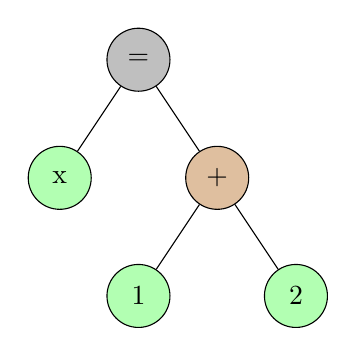
\begin{tikzpicture}[
  level distance=1.5cm,
  sibling distance=2cm,
  every node/.style={circle,draw,minimum size=0.8cm},
  root/.style={fill=gray!50},
  internal/.style={fill=brown!50},
  leaf/.style={fill=green!30}
]
  \node[root] {=}
    child { node[leaf] {x} }
    child { node[internal] {+}
      child { node[leaf] {1} }
      child { node[leaf] {2} }
    };
\end{tikzpicture}
\end{center}

ところで、JavaScriptには\textgt{自動セミコロン挿入}（ASI: Automatic
Semicolon Insertion）というルールがあり、文末のセミコロンを書き忘れた場合に処理系が暗黙的にセミコロンを補ってくれます。一見便利な機能ですが、ASIのルールは「行終端文字の後に続くトークンが、現在の文法的文脈で許されない場合に限り、行終端文字の位置にセミコロンを挿入する」というもので、時として直感に反する結果を生みます。

たとえば、上記のコードと一見似ている次の例は、実は
\textbf{\sffamily ASI}\textgt{が効かない} ためそのまま \texttt{x\ =\ 1\ +\ 2}
と解釈されます。

\begin{codescreen}{}
x = 1
+ 2
\end{codescreen}

\texttt{x\ =\ 1} の次の行が \texttt{+} で始まっていても、\texttt{+}
は二項演算子として前の式の継続と見なせるため、ASIによるセミコロン挿入は起こらないのです。

一方、\texttt{return}文の直後で改行すると、ASIが効いて意図しない結果になります。

\begin{codescreen}{}
return
a + b;
\end{codescreen}

これは \texttt{return;\ a\ +\ b;} と解釈され、関数は \texttt{undefined}
を返してしまいます。\texttt{return}
の直後にどんなトークンが来ても文として続けられないため、ASIが発動するのです。さらに、次のような行頭の
\texttt{[} も典型的な落とし穴です。

\begin{codescreen}{}
var a = 1, b = 2
b
[a, b].forEach(x => console.log(x))  // b[a, b].forEach(...) と解釈される
\end{codescreen}

\texttt{b} の次に \texttt{{[}} が来ても、\texttt{b{[}...{]}}
というインデックスアクセスとして文を継続できてしまうため、ASIは発動せず、意図と異なる解析結果になります。このような複雑さは、構文解析器の実装を難しくする一因となります。ASIによる予期せぬ挙動を避けるために、行頭にセミコロンを記述するスタイル（いわゆるセミコロン前置記法）を採用する開発者もいます。

2000年以降に登場して普及した言語は、このような特徴を持っていることが多いです。たとえば、Go、Swift、Kotlin、Scalaの文法はこのような特徴を持っています。より古い言語であるRubyやPythonも同じ特徴を持っています。このように、ちょっとした違いで構文解析結果が変わってしまう例は珍しくありません。

このような文法の進化の背景には、プログラマにとって「書きやすく読みやすい」文法を提供するという意図があります。このような「改行に敏感な」文法があると、構文解析器が複雑になりがちです。プログラミング言語の設計者にとっては考慮すべき点が増えるので、このような文法を嫌う言語設計者もいますが、利用者にとってはセミコロンの入力を省略できるなどの利便性があるため、広く採用されています。

しかし「構文解析が複雑になる」というのはいったいどういうことでしょうか。ほとんどの方はピンとこないのではないでしょうか。この本では、このような問いに対して一定の答えを提示することを目指します。「構文解析の複雑さ」と一言で言っても、その要因はさまざまです。たとえば、文法が曖昧であるか（一つの文に対して複数の解釈が可能か）、解析にバックトラック（試行錯誤）が必要か、どれだけの先読みトークン（入力の一部を先に見る数）が必要か、といった要素が複雑さに関わってきます。

本書では、これらの概念に触れながら、構文解析の奥深さを探求していきます。これらの複雑さを理解する上で重要な役割を果たすのが、「文脈自由文法」という考え方です。文脈自由文法とは、簡単に言えば、プログラムの構造を定義するための一連の書き換え規則のことです。たとえば、「数値は式である」や「式は、式と演算子と式からなる」といったルールを形式的に記述するものです。詳細については第3章で詳しく解説しますが、この文脈自由文法という道具立てがあることで、構文解析のさまざまな側面を体系的に議論できるようになります。

読者の皆さんは既存の言語に歯がゆさを感じたことはないでしょうか。たとえば、昨今はJSONやYAMLを使って領域特化言語（DSL: Domain Specific Language）を提供することが一般的になっています。Amazon Web
Services（AWS）のCloudFormationやGoogle Cloud
Platform（GCP）のDeployment
Managerなどがその例です。これらのDSLは、JSONやYAMLという既存のデータ形式を利用して、特定のドメインに特化した言語を提供しています。

しかし、これらのDSLはJSONやYAMLの枠に収めるために無理をしており、どうしても「不自然」な文法になってしまいます。JSONやYAMLは世界中に普及していますから、JSONやYAMLを使ったDSLを提供する合理性はあるものの、場合によってはJSONやYAMLに縛られないDSLの文法を考案することが求められることもあります。そのためには構文解析の知識が必要です。

構文解析は単に実用的であるにとどまらず非常に「楽しい」テーマです。読者の皆さんには本書を通じて、ぜひ「構文解析の面白さ」を感じていただければと思います。

さて、序章を読み終えた皆さんは、構文解析というテーマに対してどのような印象を持たれたでしょうか。もしかしたら、「普段何気なく書いているプログラムの裏側では、こんな複雑なことが行われているのか」と驚かれたかもしれません。あるいは、「自分の手で言語のルールを定義し、それを解釈するプログラムを作るのは面白そうだ」と感じた方もいるかもしれません。あなたがこれまでに触れたことのある言語で、構文が原因で混乱した経験はありますか？もしあれば、それはなぜだったのか、この本を読み進める中でヒントが見つかるかもしれません。

次の第1章では、いよいよ具体的な構文解析の世界に足を踏み入れ、簡単な算術式を題材に、手を動かしながら構文解析の第一歩を体験していただきます。お楽しみに！


\begin{tcolorbox}[breakable,title=現代の構文解析の課題]
  構文解析技術は長い歴史を持ちますが、現代においては新たな課題に直面しています。

\begin{description}
  \item[エラーリカバリー：]
従来の構文解析器は、文法エラーに遭遇すると即座に処理を停止していました。これは、最初の文法エラーが後続の文法エラーを引き起こす上に、後続の文法エラーが実態を表していないことが多かったための措置でした。しかし、IDEでは入力途中のコードを常に解析する必要があります。そのため、エラーがあっても可能な限り解析を続行し、意味のあるエラーメッセージを提供する「エラーリカバリー」技術が重要になっています。
\item[インクリメンタル構文解析：]
ファイル全体を毎回解析し直すのは非効率です。変更された部分だけを再解析する「インクリメンタル構文解析」により、大規模なファイルでもリアルタイムな解析が可能になります。
\item[\textbf{\sffamily Language Server Protocol（LSP）}：]
Microsoftが提唱したLSPは、言語サーバーとエディタ間の通信プロトコルです。実質的にはIDEのための基盤プロトコルと言ってもよいでしょう。構文解析結果を効率的に共有することで、一つの言語サーバーが複数のエディタに対応できるようになりました。
\item[\textbf{\sffamily AI}との融合：]
GitHub CopilotやChatGPTのようなAIツールは、コードの構造を理解する必要があります。構文解析によって得られた抽象構文木は、AIがコードを\textbf{理解}するための重要な手がかりとなっています。
\end{description}

これらの課題は、構文解析が単なる「文字列から木構造への変換」以上の役割を担っていることを示しています。
\end{tcolorbox}
